%******************* START *******************
\documentclass[ms-thesis,12pt,mathdesign]{ndsu-thesis-2022}

%Refer documentation (ndsu-thesis-2022-documentation.pdf) for various options and commands

%******************* Packages, newcommands, and other customization *******************
\usepackage[style=apa,natbib=true,backend=biber]{biblatex}% works with \citep and \citet commands
\addbibresource{mybib.bib}% *.bib extension is necessary 
\renewcommand\myspacing{1.9} % 23 lines/page needs 1.9 for thesis

%***** SI units setup and a few custom unit commands *****
\sisetup{group-separator = {,}}% thousands separator comma; space default
\DeclareSIUnit\gal{gallon}
\DeclareSIUnit\ft{ft}
\newcommand{\sqft}[1]{\qty{#1}{foot}$^2$\xspace}% have math outside of SI
\newcommand{\cuft}[1]{\qty{#1}{\cubic\ft}\xspace}% SI standard commands
 
%******************* First and second page material *******************
\title{The Title of My M.S. Thesis}
\author{Samuel Fargo Bison}
\date{December 2023}
\progdeptchoice{Department} % Use Department (or) Program
\department{Mathematics}

\cchair{Prof. John Adams} % Use actual committee members names 
\cmembera{Prof. Abraham Lincoln}
\cmemberb{Prof. George Washington}
\cmemberc{Prof. Theodore Roosevelt} % If 3rd not required - delete this line 
\approvaldate{12/14/2022}
\approver{Prof. James Garfield}

%******************* Front matter *******************
\abstract{This is the abstract for my thesis. \\ \emph{Abstracts for doctoral dissertations must use 350 words or less. Abstracts for master's papers or master's theses must use 150 words or less.}\\ \kant[16]}% dummy text

\acknowledgements{I acknowledge people here. \\ \emph{Acknowledgements text should be placed here.} \\ \kant[15]}

\dedication{This thesis is dedicated to my cat, Mr. Fluffles.\\ \emph{This section dedicates the disquisition to a few significant people. The text must be double-spaced and aligned center to the page.} \\ Which is already taken care of by this \LaTeX\ class.}

\preface{You can put a preface here. \\ \emph{This section is optional!} \\ \kant[14]}

\listofabbreviations{% may use title case
AC          	& alternating current \\
NDSU     	& North Dakota State University \\
ZL       	& zeta level}

\listofsymbols{% may use sentence case
$A$     	& area (\unit{\m\squared})\\
$e$     	& Euler's constant (\num{2.718281828}) \\
$R^2$   	& coefficient of determination}

%******************* Document start *******************
\begin{document}

%******************* First chapter - paper style *******************
\mypaperheading{The First Chapter - Paper Style - Long title of this technical paper}{This paper is planned to be submitted as a peer-reviewed article \ldots\ more information about the author(s),  title,  \emph{journal},  to be added.}

%------------------------------------------------------
\section{Abstract}
Paper-styled chapters will have abstracts. Abstract of this chapter goes here. \kant[1]

%------------------------------------------------------
\section{Section ($\Rightarrow$ 1st level; Title Case; Centered; Boldface)}
This is the first section of the thesis (1st level: 1.2. Section). \kant[2]

%------------------------------------------------------
\section{Section}
This is the second section of the thesis (1st level: 1.3. Section). \kant[3]

%------------------------------------------------------
\subsection{Subsection ($\Rightarrow$ 2nd level; Title Case; Left-justified; Boldface)}
This is the subsection text (2nd level: 1.3.1. Subsection). \kant[4]

%------------------------------------------------------
\subsubsection{Subsubsection ($\Rightarrow$ 3rd level; Title Case; Left-justified; Boldface; Italics)}
This is the subsection text (3rd level: 1.3.1.1. Subsubsection). \kant[5]

%------------------------------------------------------
\paragraph{Paragraph ($\Rightarrow$ 4th level; Sentence case; Left-justified; No bold; Italics)}
This is the subsection text (4th level: 1.3.1.1.1. Paragraph). \kant[6]

%------------------------------------------------------
\subparagraph{Subparagraph ($\Rightarrow$ 5th level; Sentence case; Left-justified; No bold; Regular)}
This is the subsection text (5th level: 1.3.1.1.1.1. Paragraph). \kant[7]

%------------------------------------------------------
\section{Table and Figure}
This is the third section of the thesis (1st level: 1.4. Section). This section illustrates the inclusion of a simple table (\cref{tab:1}) and a figure shown later.

\begin{table}[h]
\centering
\caption{Table captions go at the top of the table. This was a long caption of the table included in the first chapter --- so that we see how it breaks into another line and has a single spacing. Usually, tables are of full-width and are demonstrated subsequently.}
\vspace{-1ex}
\begin{tabular}{clr}
\toprule
Number & Month & Days\\
\midrule
\#1 & January    & 31\\
\#2 & February   & 28\\
\#3 & March      & 31\\
\bottomrule
\end{tabular}
\label{tab:1}
\end{table}	\kant[7]

Now the figure (\cref{fig:1}) illustrates an example figure from the \texttt{mwe} package.

\myfig{H}{0.525}{example-image-duck}{Caption for this example image in this first chapter.}{fig:1}	
\kant[8-9]

%******************* Second chapter - regular *******************
\myheading{The Second Chapter - Regular Style - Long title for this chapter}

Regular style chapters will not have abstracts. General information or outline of the chapter is given here --- before breaking into sections. 

%------------------------------------------------------
\section{Excellent Results}
This is another section of the thesis (1st level: 2.1. Experimental Results).\Cref{tab:2} presents the results in a tabular form that spans the entire width. Please note the results shown (\cref{tab:2}) are preliminary.

\begin{table}[ht]
\centering
\caption{Table spanning entire width (full-width) using \texttt{setlength} and
\texttt{tabcolsep}.}
\vspace{-1ex}
\setlength{\tabcolsep}{3.75em}
\begin{tabular}{@{\hspace{2ex}} lccr @{\hspace{2ex}}}
\toprule
Number & Name of month & Days & Season\\
\midrule
\#4 	& April  & 30		& Spring\\
\#5 	& May    & 31		& Summer\\
\#6 	& June   & 30		& Summer\\
\bottomrule
\end{tabular}
\begin{tablenotes}[flushleft]
\item \hspace{-1ex} Note: The \texttt{tablenotes} environment produces table footnotes. 
\end{tablenotes}
\label{tab:2}
\end{table}	\kant[7-8]

%------------------------------------------------------
\subsection{Minor Results}
This is a subsection of the thesis (1st level: 2.2. Experimental Results). 	

\kant[8]
The \Cref{fig:2} is an example image with command showing all arguments including the optional caption placement. The example figure (\cref{fig:2}) is included in the \texttt{mwe} package.

\myfig[2ex]{H}{0.35}{example-image}{Caption for this example image demonstrating an optional 2ex vertical spacing. Compare this with a narrow caption spacing without optional argument in 
\cref{fig:1}.}{fig:2}
\kant[8]

%------------------------------------------------------
\section{Equations}
\kant[2]

\myeqn{% shortcut for equation vertically spaced
y = (mx + c) \times \text{NCF} \times S_\text{factor} \times c_p \times M_\text{p}
\label{eq:lin}
}

\noindent where $y$ is the dependent variable, $m$ is the slope, $x$ is the independent variable, $c$ is the $y$ intercept, NCF is the normalized conversion factor, $S_\text{factor}$ is the scale factor, $c_p$ is the specific heat capacity at constant pressure ($p$, variable), and $M_\text{p}$ is the mass of a proton (p, descriptive). 

Note how variables, abbreviations, and subscripts are coded in \cref{eq:lin}. Refer Extended Thesis to know more about equations and shortcuts. 

%------------------------------------------------------
\section{Schemes}
\kant[2]

The regular way of coding a scheme:

\begin{scheme}
\centering
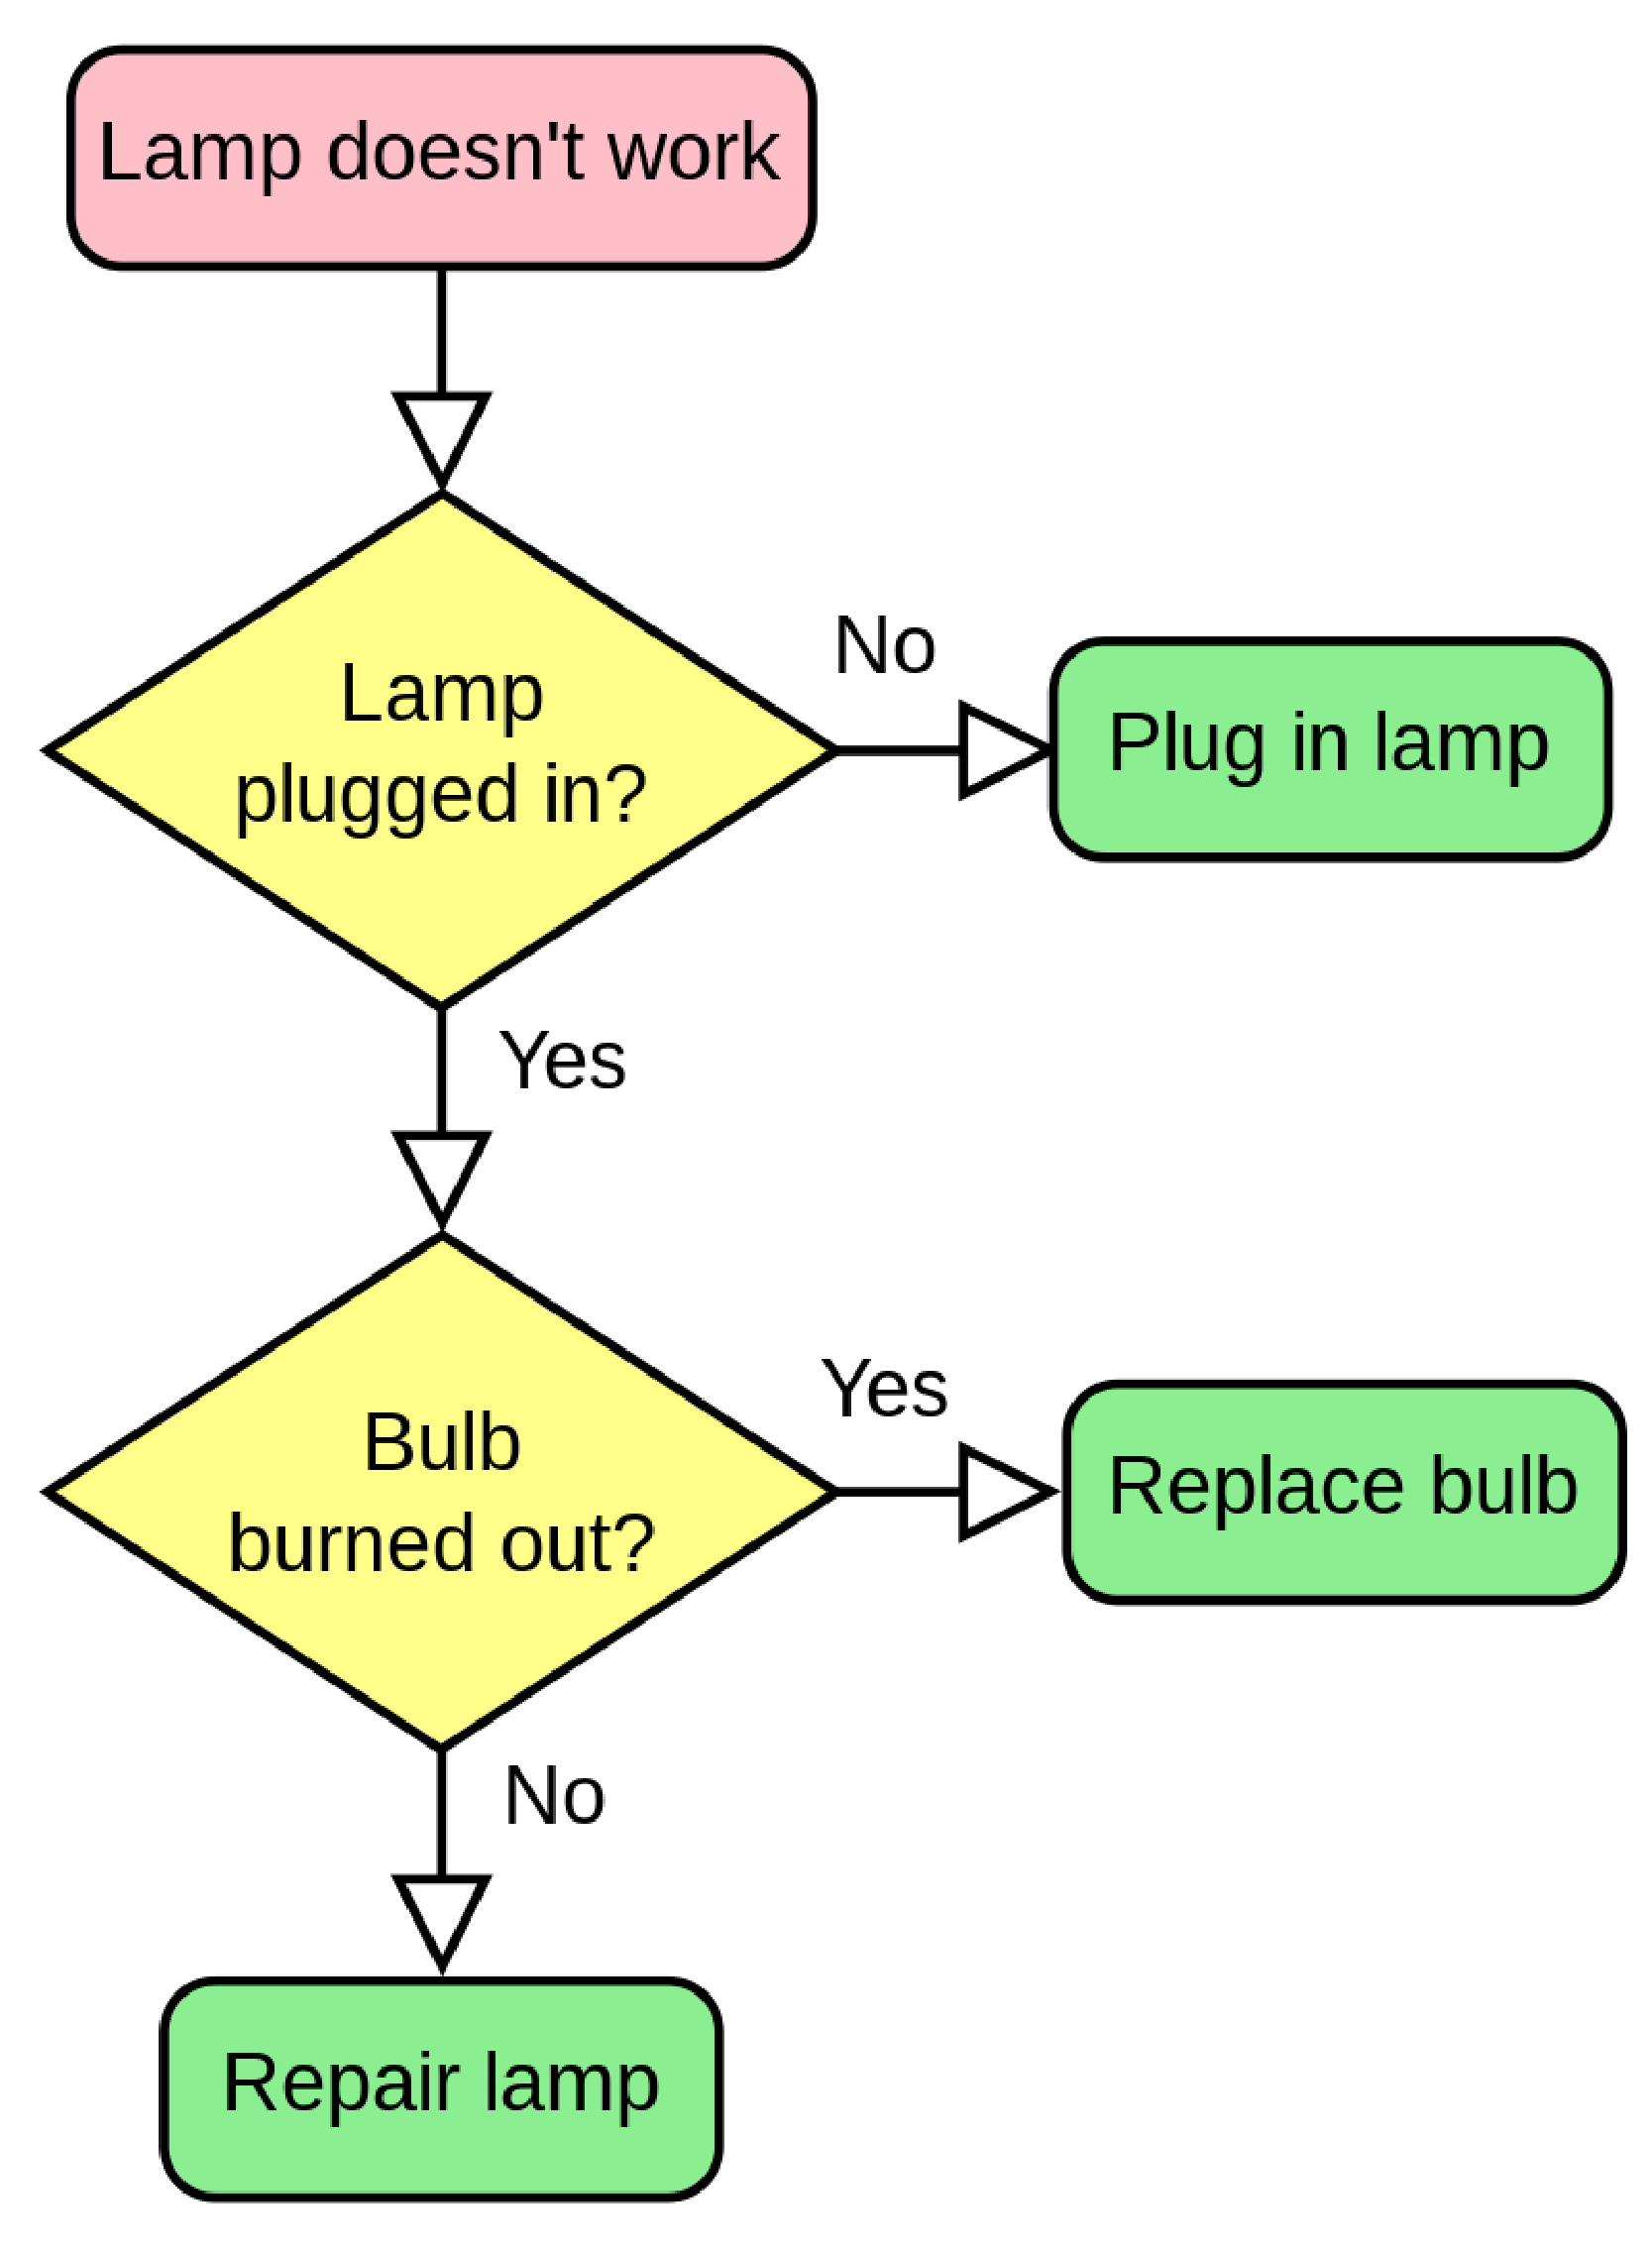
\includegraphics[width=0.4\textwidth]{LampFlowchart}
\caption{Flowchart of controls of light bulb --- A scheme}
\label{sc1}
\end{scheme}
%

\kant[9]\vspace{-1.5ex}

\mysch[2ex]{h!}{0.48}{LampFlowchart}{Caption for this example image demonstrating an optional 2ex vertical spacing. Compare this with a narrow caption spacing without optional argument in \cref{fig:2}.}{sc2}

\kant[2]\kant[9]

The (\cref{sc1,sc2}) are good. And, stating this differently all the \Cref{sc1,sc2,sc3} are good too. Note that \Cref{sc3} is in landscape mode.

\myschls[1ex]{p}{0.65}{LampFlowchart}{Landscape scheme --- Flowchart of controls of light bulb. Optional 2ex vertical spacing was used.}{sc3}


%------------------------------------------------------
\section{Some References}
Referring to all entries in the ``\texttt{mybib.bib}'' file to generate the citations here and the listing using the \texttt{\textbackslash citep\{\ldots\}} ``natbib'' command (cite parenthesis \citep{texbook,lcompanion,latex2e,knuth1984,lesk1977,amsthm2017,calvo2004using,cannayen2011latex,kopka2004guide,notso2021,bari2016identification}.

The same using \texttt{\textbackslash citet\{\ldots\}} command (cite text) in the running text as: The authors \citet{texbook,lcompanion,latex2e,knuth1984,lesk1977,amsthm2017,calvo2004using,cannayen2011latex,kopka2004guide,notso2021,bari2016identification} have something to do with \LaTeX. For most bibliography citations and list creation, these two commands are sufficient.

%-----------------------------------------------------------------------------


%******************* Bibliography handling *******************
\makerefs %For individual chapter references - command should be inside refsection environment


%******************* Named appendix A *******************
\namedappendices{A}{Named first appendix}
Appendix material can be included here. First a paragraph of text and then an example figure (fig.~\ref{fig:ap1}).

%------------------------------------------------------
\section{Appendix A - Section With Figure}
\kant[9]
\myfigap{H}{0.5}{example-image-golden}{A golden ratio rectangle image.}{fig:ap1}	\kant[8]

\section{Appendix A - Section With Table}
And, then including a table (table.~\ref{tab:ap1}).

\begin{appendixtable}[h]
\centering
\caption{Use of \texttt{tblr} environment for full-width table - applicable to both main text 
and appendix.  Note the use of \texttt{booktabs} commands and `X' parameters to reproduce 
Table~\ref{tab:2}.}
\begin{tblr}{*4X}
\toprule
Number 	& Name of month 	& Days 	& Season\\
\midrule
\#7 			& July       		& 30 		& Spring\\ \cmidrule[lr]{2-4}
Multicolumn 	&\SetCell[c=3]{c} The three columns combined \\ \cmidrule[lr]{2-4}
\#8 			& August 		 & 31 	& Summer\\
\#9 			& September 	& 30 		& Summer\\
\bottomrule
\end{tblr}
\begin{tablenotes}[flushleft]
\item \hspace{-1ex} Note: The \texttt{tablenotes} environment produces table footnotes. Refer to \texttt{tabularray} documentation for further details.  
\end{tablenotes}
\label{tab:ap1}
\end{appendixtable}

For other types of tables and figures, such as landscape tables, long tables, landscape long tables, landscape figures, subfigures, subfigures spanning multiple pages, and multiple figures in landscape see NDSU-Thesis-Extended code and output. 

%------------------------------------------------------
\subsection{Appendix A Subsection}
\kant[10]


%******************* Named Appendix B *******************
\namedappendices{B}{Named second appendix}
Appendix material can be included here. First including a figure (fig.~\ref{fig:ap2}).

%------------------------------------------------------
\section{Appendix B - Section With Figure}
\kant[9]
\myfigap[0.5ex]{H}{0.6}{example-grid-100x100pt}{A $10 \times 10$ grid of different concentric colors.}{fig:ap2}

%------------------------------------------------------
\section{Appendix B - Section With Table}
Now coding another appendix table (table.~\ref{tab:ap2}) that spans the entire width using the manual method (using `tabcolsep' command; and `resize' command to fit large tables).

\begin{appendixtable}[h]
\centering
\caption{Squares and cubes in named appendix table using \texttt{siunitx} and \texttt{tabularray} 
packages.}
\begin{tblr}{X X[c] X[r] X[1.5,r]}
\toprule
Number & Square        & Cubes          & Fourth power\\
\midrule
11 	   & 121   			        & \num{1331} 		   & \num{14641}\\
22 	   & 484  			        & \num{10648}		   & \num{234256}\\
333 	   & \num{110889}             & \num{36926037}	   & \num{12296370321}\\
\bottomrule
\end{tblr}
\label{tab:ap2}
\end{appendixtable}
 
%------------------------------------------------------
\subsection{Appendix B Subsection}
\kant[11]

\closeappendices  % Refer documentation Table 3 for proper closing 

\end{document}
%******************* END *******************